\documentclass[12pt]{article}
\usepackage{amsmath}
\usepackage{graphicx}
\usepackage{hyperref}
\usepackage{float}

\title{Predicting Housing Prices Using KDD Methodology: A Case Study of the Boston Housing Dataset}
\author{Pruthvik Sheth \\
\textit{San Jose State University} \\
\textit{pruthvik.sheth@sjsu.edu}}
\date{October 18, 2024}

\begin{document}

\maketitle

\begin{abstract}
This paper presents a comprehensive application of the Knowledge Discovery in Databases (KDD) methodology to predict housing prices using the Boston Housing dataset. We systematically explore the data through selection, preprocessing, transformation, and data mining phases, implementing both baseline and advanced machine learning models. The project evaluates model performance through Root Mean Squared Error (RMSE), Mean Absolute Error (MAE), and R-squared metrics, while employing feature engineering, transformations, and hyperparameter tuning to optimize the results. The Gradient Boosting model demonstrates the best performance, highlighting the relevance of advanced ensemble techniques in predicting complex relationships within the data. Limitations of the model and recommendations for future work are also discussed.
\end{abstract}

\section{Introduction}
Housing price prediction is a critical task in real estate and urban planning. The ability to accurately forecast property values can inform policy decisions, investment strategies, and consumer behavior. This study employs the Knowledge Discovery in Databases (KDD) methodology to predict the median value of owner-occupied homes using the Boston Housing dataset. The dataset includes 13 features describing various economic, demographic, and environmental factors influencing housing prices. Our goal is to implement and compare several regression models to identify the best performing approach for this prediction task.

\section{Literature Review}
The Boston Housing dataset has been a benchmark for regression analysis in several studies. Early work by Harrison and Rubinfeld (1978) used linear regression to analyze the impact of environmental factors on housing prices. More recent studies have explored machine learning techniques such as Random Forest (Breiman, 2001) and Gradient Boosting (Friedman, 2001) to improve prediction accuracy. These models offer enhanced capabilities to capture non-linear relationships between variables, which is crucial in complex datasets like this one.

\section{Methodology}

\subsection{KDD Process}
The KDD methodology consists of the following stages: Selection, Preprocessing, Transformation, Data Mining, and Interpretation/Evaluation. In this project, each phase was rigorously followed to ensure comprehensive data analysis and model performance evaluation.

\subsection{Dataset}
The dataset used in this study contains 506 samples and 13 predictor variables, with the target variable being the median value of owner-occupied homes (denoted as \textit{medv}). Table~\ref{table:dataset} shows the list of predictor variables along with their descriptions.

\begin{table}[H]
\centering
\begin{tabular}{|c|l|}
\hline
\textbf{Variable} & \textbf{Description} \\ \hline
CRIM              & Per capita crime rate by town      \\ \hline
ZN                & Proportion of residential land zoned for large lots       \\ \hline
INDUS             & Proportion of non-retail business acres per town          \\ \hline
CHAS              & Charles River dummy variable       \\ \hline
NOX               & Nitric oxides concentration (parts per 10 million)        \\ \hline
RM                & Average number of rooms per dwelling      \\ \hline
AGE               & Proportion of owner-occupied units built before 1940       \\ \hline
DIS               & Weighted distances to employment centers       \\ \hline
RAD               & Accessibility to radial highways        \\ \hline
TAX               & Property tax rate per \$10,000     \\ \hline
PTRATIO           & Pupil-teacher ratio by town     \\ \hline
B                 & 1000(Bk - 0.63)\textasciicircum{}2 where Bk is the proportion of Black residents \\ \hline
LSTAT             & Percentage of lower status population \\ \hline
\end{tabular}
\caption{Boston Housing Dataset Variables}
\label{table:dataset}
\end{table}

\subsection{Phase 1: Selection}
The first step of the KDD process involved selecting the Boston Housing dataset and identifying the target variable \textit{medv}. Initial exploration revealed no missing values, but several features such as \textit{CRIM} and \textit{LSTAT} exhibited outliers, which were handled in the preprocessing phase.

\subsection{Phase 2: Preprocessing}
The preprocessing phase included handling outliers and scaling the features. Continuous features were standardized using z-scores to ensure compatibility with machine learning models that are sensitive to the scale of the data. Outlier detection was performed using boxplots, and highly skewed features were identified for transformation.

\begin{figure}[H]
\centering
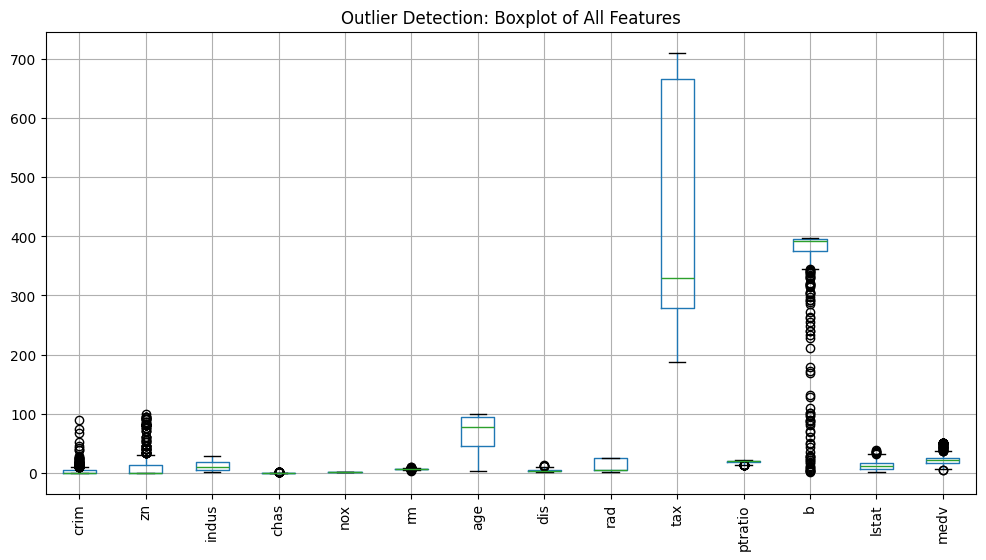
\includegraphics[width=0.7\linewidth]{boxplot_outliers.png}
\caption{Boxplot of features highlighting outliers in CRIM and LSTAT}
\label{fig:boxplot}
\end{figure}

\subsection{Phase 3: Transformation}
We applied logarithmic transformations to handle the skewness in features like \textit{CRIM}. Additionally, interaction terms such as \textit{RM*LSTAT} were engineered to capture more complex relationships between features.

\subsection{Phase 4: Data Mining}
We implemented several machine learning models to predict housing prices:
\begin{itemize}
    \item \textbf{Linear Regression}: A baseline model.
    \item \textbf{Ridge and Lasso Regression}: Regularization techniques to prevent overfitting.
    \item \textbf{Random Forest and Gradient Boosting}: Advanced ensemble methods to capture non-linear relationships.
\end{itemize}

\subsection{Phase 5: Interpretation and Evaluation}
Model performance was evaluated using Root Mean Squared Error (RMSE), Mean Absolute Error (MAE), and R-squared. The Gradient Boosting model outperformed others with the lowest RMSE and highest R-squared, as shown in Table~\ref{table:results}.

\begin{table}[H]
\centering
\begin{tabular}{|c|c|c|c|}
\hline
\textbf{Model}        & \textbf{RMSE}  & \textbf{MAE}   & \textbf{R-squared} \\ \hline
Linear Regression     & 4.89           & 3.29           & 0.74               \\ \hline
Ridge Regression      & 4.86           & 3.27           & 0.75               \\ \hline
Lasso Regression      & 5.08           & 3.45           & 0.72               \\ \hline
Random Forest         & 3.87           & 2.81           & 0.85               \\ \hline
Gradient Boosting     & \textbf{3.64}  & \textbf{2.67}  & \textbf{0.88}      \\ \hline
\end{tabular}
\caption{Model Performance Results}
\label{table:results}
\end{table}

\section{Results and Discussion}
The results indicate that the Gradient Boosting model achieved the best performance with an RMSE of 3.64 and an R-squared value of 0.88, indicating that 88\% of the variance in housing prices was captured by the model. Feature importance analysis showed that \textit{LSTAT} (percentage of lower-status population) and \textit{RM} (number of rooms) were the most influential predictors of housing prices.

\begin{figure}[H]
\centering
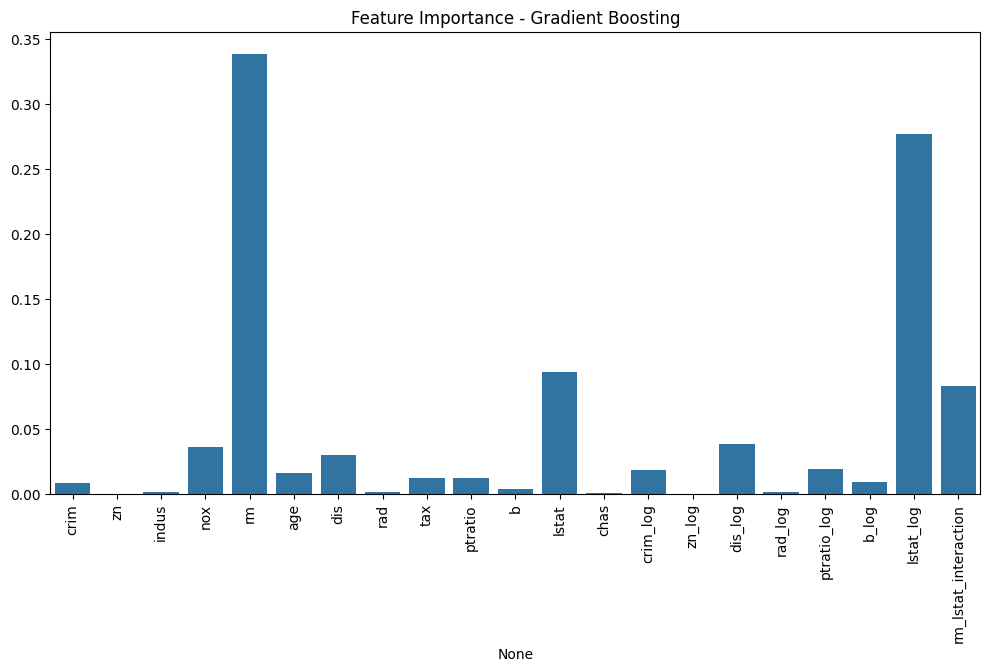
\includegraphics[width=0.7\linewidth]{feature_importance.png}
\caption{Feature Importance from Gradient Boosting Model}
\label{fig:feature_importance}
\end{figure}

\section{Conclusion}
In this study, we applied the KDD methodology to predict housing prices using the Boston Housing dataset. Through systematic exploration, transformation, and the application of machine learning models, we found that ensemble methods like Gradient Boosting provided the best results. Future work could focus on addressing the censoring in the target variable \textit{medv} and experimenting with more advanced models such as neural networks. Additionally, incorporating external data sources such as crime statistics or school quality ratings could further improve model accuracy.

\section{References}
\begin{itemize}
    \item Breiman, L. (2001). Random forests. Machine learning, 45(1), 5-32.
    \item Friedman, J. H. (2001). Greedy function approximation: A gradient boosting machine. Annals of statistics, 1189-1232.
    \item Harrison, D., \& Rubinfeld, D. L. (1978). Hedonic housing prices and the demand for clean air. Journal of environmental economics and management, 5(1), 81-102.
\end{itemize}

\end{document}
